\documentclass[10pt]{article}

\usepackage[a4paper,margin=0.58in]{geometry}
\usepackage{amsmath}
\usepackage{graphicx}

\graphicspath{{figures/}}
\setlength{\parskip}{3pt}
\setlength{\parindent}{1em}
\setlength{\textfloatsep}{5pt plus 1pt minus 1pt}
\setlength{\intextsep}{5pt plus 1pt minus 1pt}
\setlength{\floatsep}{5pt plus 1pt minus 1pt}

\makeatletter
\renewcommand\section{\@startsection{section}{1}{\z@}%
  {1.5ex plus .4ex minus .2ex}{.5ex plus .1ex}%
  {\normalfont\large\bfseries}}
\makeatother

\newcommand{\SNR}{\mathrm{SNR}}
\newcommand{\SNReff}{\mathrm{SNR}_{\mathrm{eff}}}
\newcommand{\CRB}{\mathrm{CRB}}

\title{\vspace{-1.2em}\bfseries Broadband Transient Localization over WDM Fibre:\\
Per-Pair Limits and Empirical Fusion}
\author{Author names and affiliations to be added}
\date{}

\begin{document}
\maketitle
\vspace{-2.1em}

\begin{abstract}
We study range estimation from the wavelength-dependent polarization signature of a short transient in a wavelength-division-multiplexed (WDM) fibre. Chromatic dispersion maps range to relative channel delay. We derive a two-sensor effective-SNR Cram\'er--Rao bound (CRB) for each pair, then evaluate channel selection, dispersion weighting, robust fusion, and delay-estimator bias in Monte Carlo simulations. On an equispaced grid, all-pair $D^2$ weighting is close to hard-filtered equal averaging, while robust fusion can give further gains. An alternating band-edge grid behaves differently because its low-dispersion pairs receive almost no $D^2$ weight. Pair estimates share channels and are correlated, so fused performance is reported empirically rather than as a combined CRB.
\end{abstract}

\section{Problem and contribution}
Distributed fibre sensing can detect mechanical disturbances through changes in the received state of polarization (SOP) \cite{he2021das}. When a transient has a measurable, temporally identifiable signature in several WDM channels, chromatic dispersion (CD) makes the signatures arrive at different times. For channels $i$ and $j$, let $d_i$ and $d_j$ be their CD delay per unit distance; then the signed relative-delay slope is $\Delta d_{ij}=d_i-d_j$, the pair delay at range $Z$ is $\tau_{ij}=Z\Delta d_{ij}$, and a measured delay gives $\hat Z_{ij}=\hat\tau_{ij}/\Delta d_{ij}$. Thus wavelength diversity supplies multiple range-sensitive pairs, but not independent measurements: pairs that share a channel also share its noise and waveform-specific errors.

This study addresses three distinct questions: the timing limit for one pair, how channel placement changes that pair's distance sensitivity, and how to combine the correlated pair estimates. The CRB answers the first; Monte Carlo RMSE, bias, and spread assess fusion. We do not claim that summing pairwise CRBs gives a multichannel bound. The method is scoped to events with a detectable common cross-channel signature; it is not validated for arbitrary event types.

\section{Model and per-pair timing limit}
The simulated SOP is represented by two real Stokes components. A transient modulates a local PMD section of length $0.5$\,km, centered $500$\,km from the receiver; the remaining path contributes deterministic wavelength-dependent CD delays, not a distributed PMD cascade. This isolates the local perturbation response from long-path CD. The observation model follows standard delay-estimation and PMD treatments \cite{weiss1983,sadler2006survey,gisin1992}.

For two noisy records, the frequency-bin information depends on both channels' SNRs. At frequency $f$, their effective SNR is $\SNReff(f)=\rho_i(f)\rho_j(f)/[1+\rho_i(f)+\rho_j(f)]$. For equal channels it is $\rho^2/(1+2\rho)$: approximately $\rho^2$ at low SNR, when both observations must contain signal, and $\rho/2$ at high SNR, when neither channel is a noiseless timing reference. Each bin contributes in proportion to $(2\pi f)^2\SNReff$; the contributions from both independent SOP components and all frequency bins add to the pair information $J_{ij}$. Thus $\operatorname{Var}(\hat\tau_{ij})\ge 1/J_{ij}$, and the corresponding range standard deviation is $1/(|\Delta d_{ij}|\sqrt{J_{ij}})$. The frequency weighting makes broadband temporal structure especially useful for timing \cite{weiss1983,sadler2006survey}.

The clean simulated records supply the signal spectra; the selected noise variance sets the per-bin noise powers. The CRB is therefore a model-based reference, not a fit to a measured delay error or cross-correlation peak. In a controlled two-component Gaussian-pulse check, simulated pair-delay spread was within about 4\% of the CRB at 60\,dB energy SNR. In a representative production cell, the median pair spread was 1.43 times the per-pair CRB standard deviation (10th--90th percentiles: 1.08--1.87), reflecting waveform variation and estimator effects.

\section{Pair selection and fusion}
For a set of pair range estimates, equal fusion uses $w_{ij}=1$. Since a fixed timing error maps to a smaller range error for larger $|\Delta d_{ij}|$, dispersion weighting uses $w_{ij}=D_{ij}^2$, where $D_{ij}$ is the integrated CD magnitude in ps/km. This is an inverse-marginal-variance heuristic under comparable pair timing errors, not a covariance-aware optimum. A hard filter retains pairs satisfying $D_{ij}^2\ge\alpha\max D^2$; the default $\alpha=0.25$ is equivalent to retaining pairs with $|D_{ij}|\ge0.5D_{\max}$.

Robust fusion multiplies the geometry weight by a Tukey-bisquare residual weight: $w_{ij}=D_{ij}^2\psi(r_{ij})$, where $r_{ij}$ is the distance from the pair estimate to the pool median, $s=1.5\,\mathrm{IQR}$, and $\psi(r)=[1-(r/(2.5s))^2]^2$ for $r<2.5s$ and zero otherwise. Thus $D^2$ favors pairs that are more distance-sensitive, while the residual factor suppresses pair estimates that disagree with the observed consensus. Robust fusion can help when most pairs form a reliable consensus, but may fail if that consensus is biased or wrong.

\section{Simulation results}
The production study used 10 independent PMD realizations and 100 noise realizations per fibre, two SOP components, and channel subsets from a 241-channel, 50-GHz master grid. Nominal envelope bandwidth and per-component energy SNR were swept; the main fusion comparisons use 5, 10, and 15 equispaced channels, with an alternating band-edge subset as contrast. RMSE includes both estimator bias and random spread. The quoted SNR crossings are interpolated point estimates; paired uncertainty intervals have not yet been calculated.

Figure~\ref{fig:fusion} summarizes the equispaced-grid comparison. For 15 channels near $B_{\rm nom}=22$\,kHz, the per-component energy SNR required for 5-km RMSE was 101.82\,dB for equal averaging over all pairs, 96.48\,dB for all-pair $D^2$ weighting, 95.05\,dB for robust all-pair fusion, and 96.55\,dB for equal averaging after the $\alpha=0.25$ filter. At this operating point, soft $D^2$ weighting is close to hard selection; robust fusion improves the crossing by about 1.5\,dB relative to filtered equal averaging. These are empirical point comparisons, not evidence that every small difference is statistically resolved.

\begin{figure}[tb]
\centering
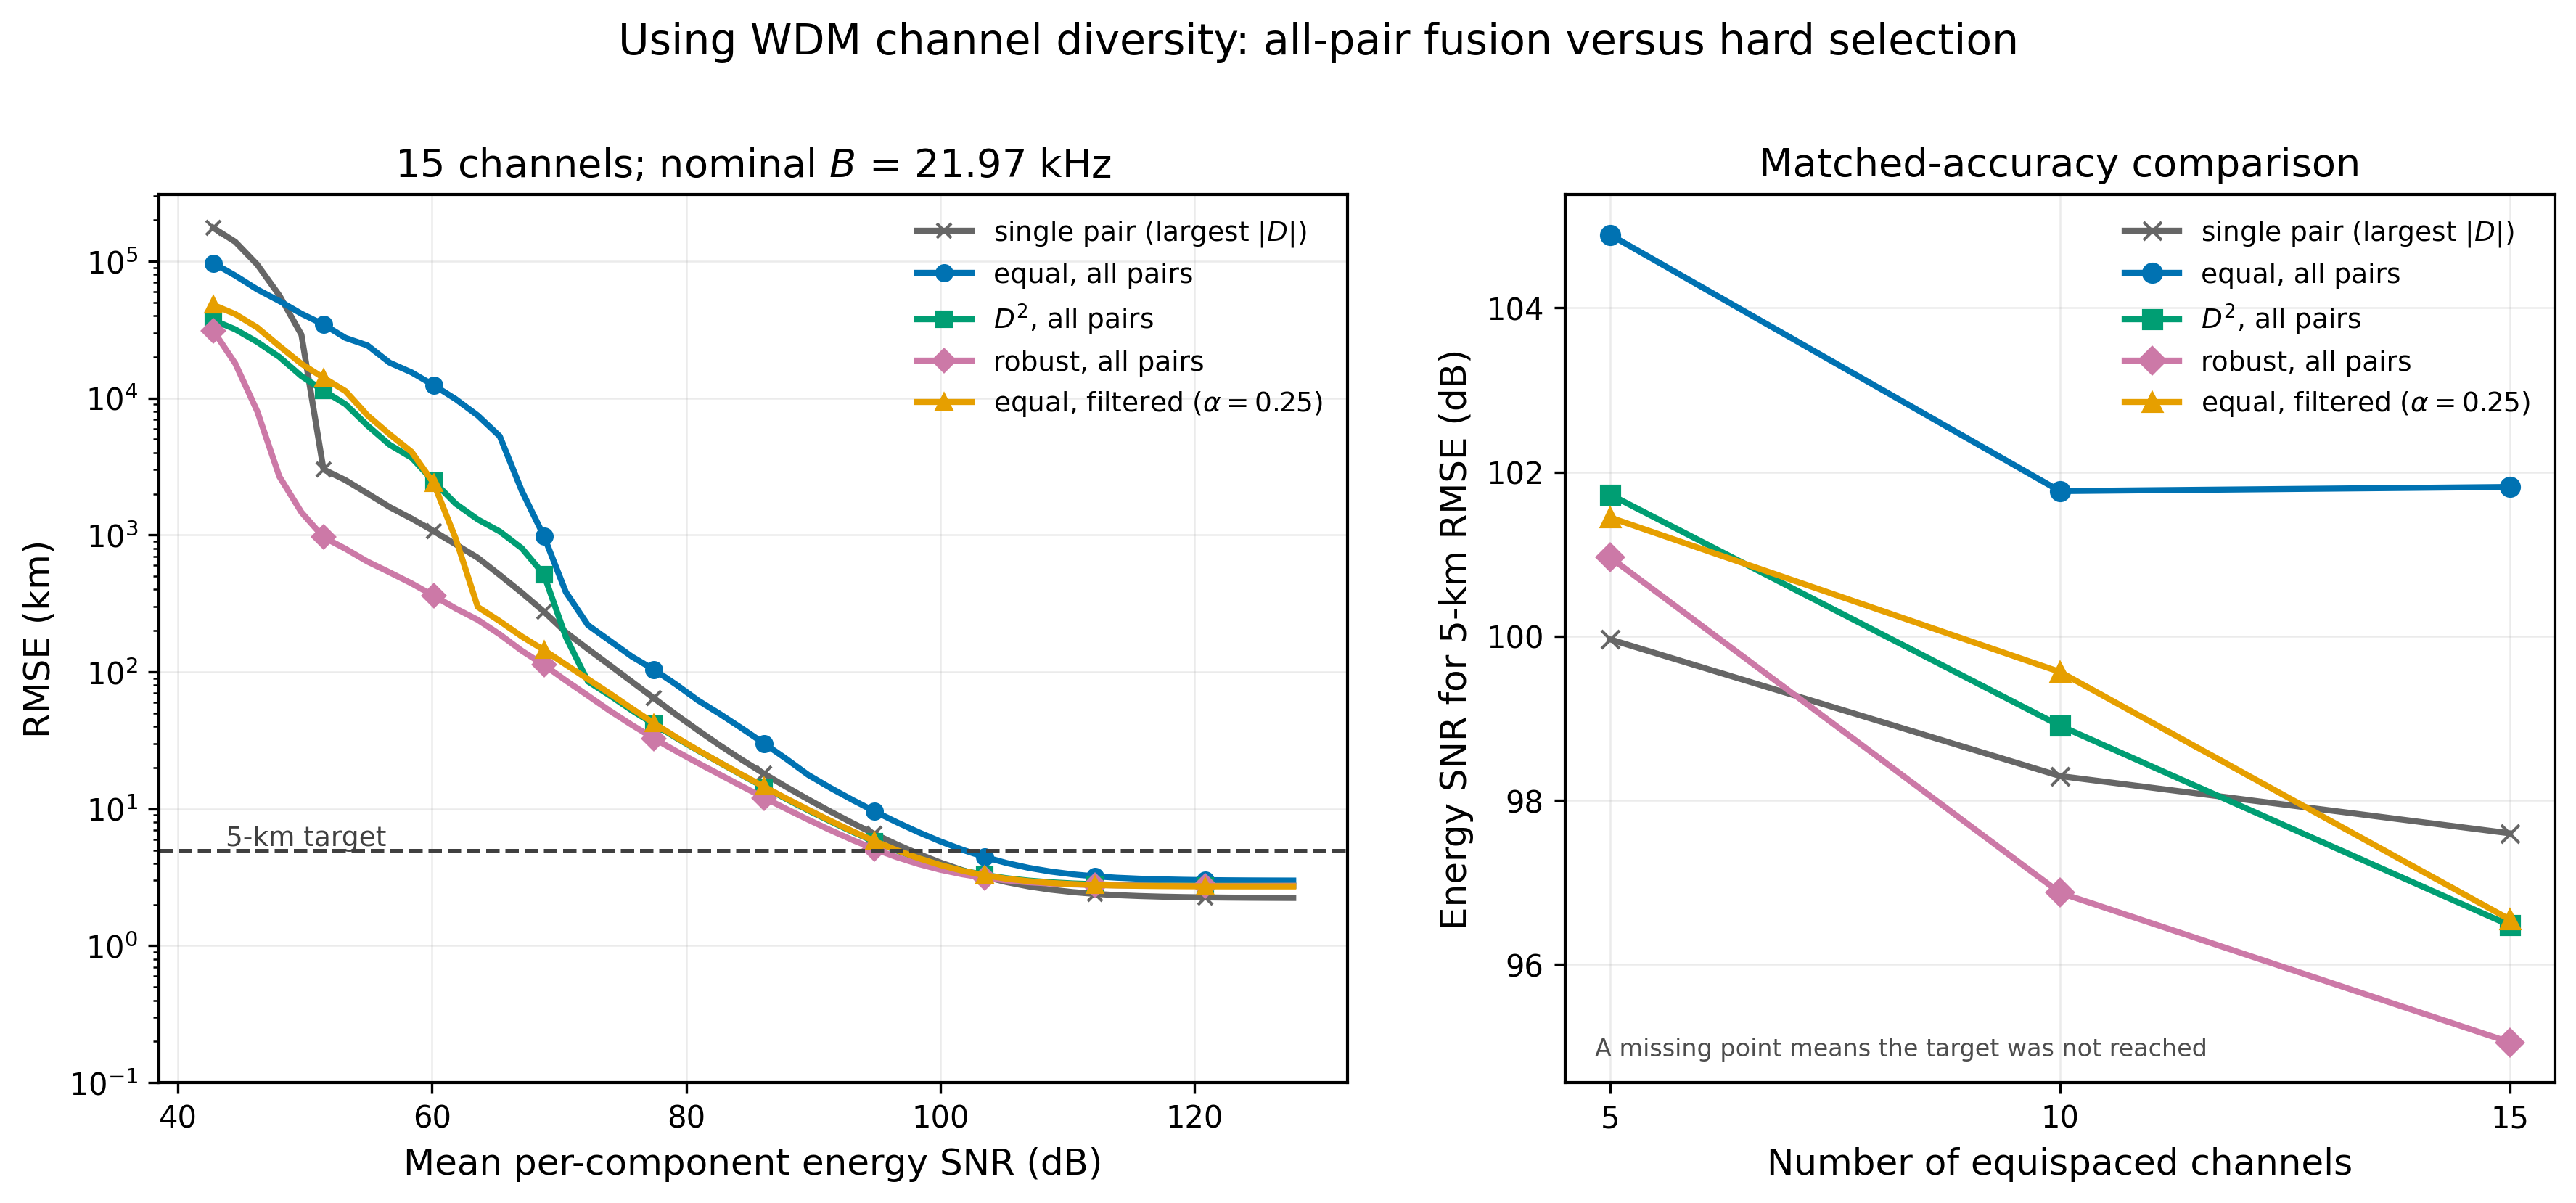
\includegraphics[width=0.90\linewidth]{F10_equispaced_fusion_strategy.png}
\caption{EQUISPACED GRID: empirical RMSE and energy SNR needed for a 5-km RMSE target as channel count increases. The best method depends on the operating point; pair estimates are correlated.}
\label{fig:fusion}
\end{figure}

The mechanism is visible in Fig.~\ref{fig:weights}. On the equispaced grid, pair dispersion varies gradually: the hard filter retains 32 of 105 pairs, while the excluded pairs still account for 26.2\% of the all-pair $D^2$ weight. On the 12-channel alternating band-edge grid, dispersion separates into low- and high-sensitivity groups; the filter retains 36 of 66 pairs, and excluded pairs have only 0.011\% of total $D^2$ weight. Consistent with this, at about 22\,kHz the band-edge 12-channel 5-km target required 119.84\,dB for equal all-pair fusion but about 90.0\,dB for $D^2$, robust, or filtered-equal fusion. Here $D^2$ weighting nearly acts as a soft version of deleting the low-dispersion group. The weight fractions describe the rule's allocation, not independent statistical information.

\begin{figure}[tb]
\centering
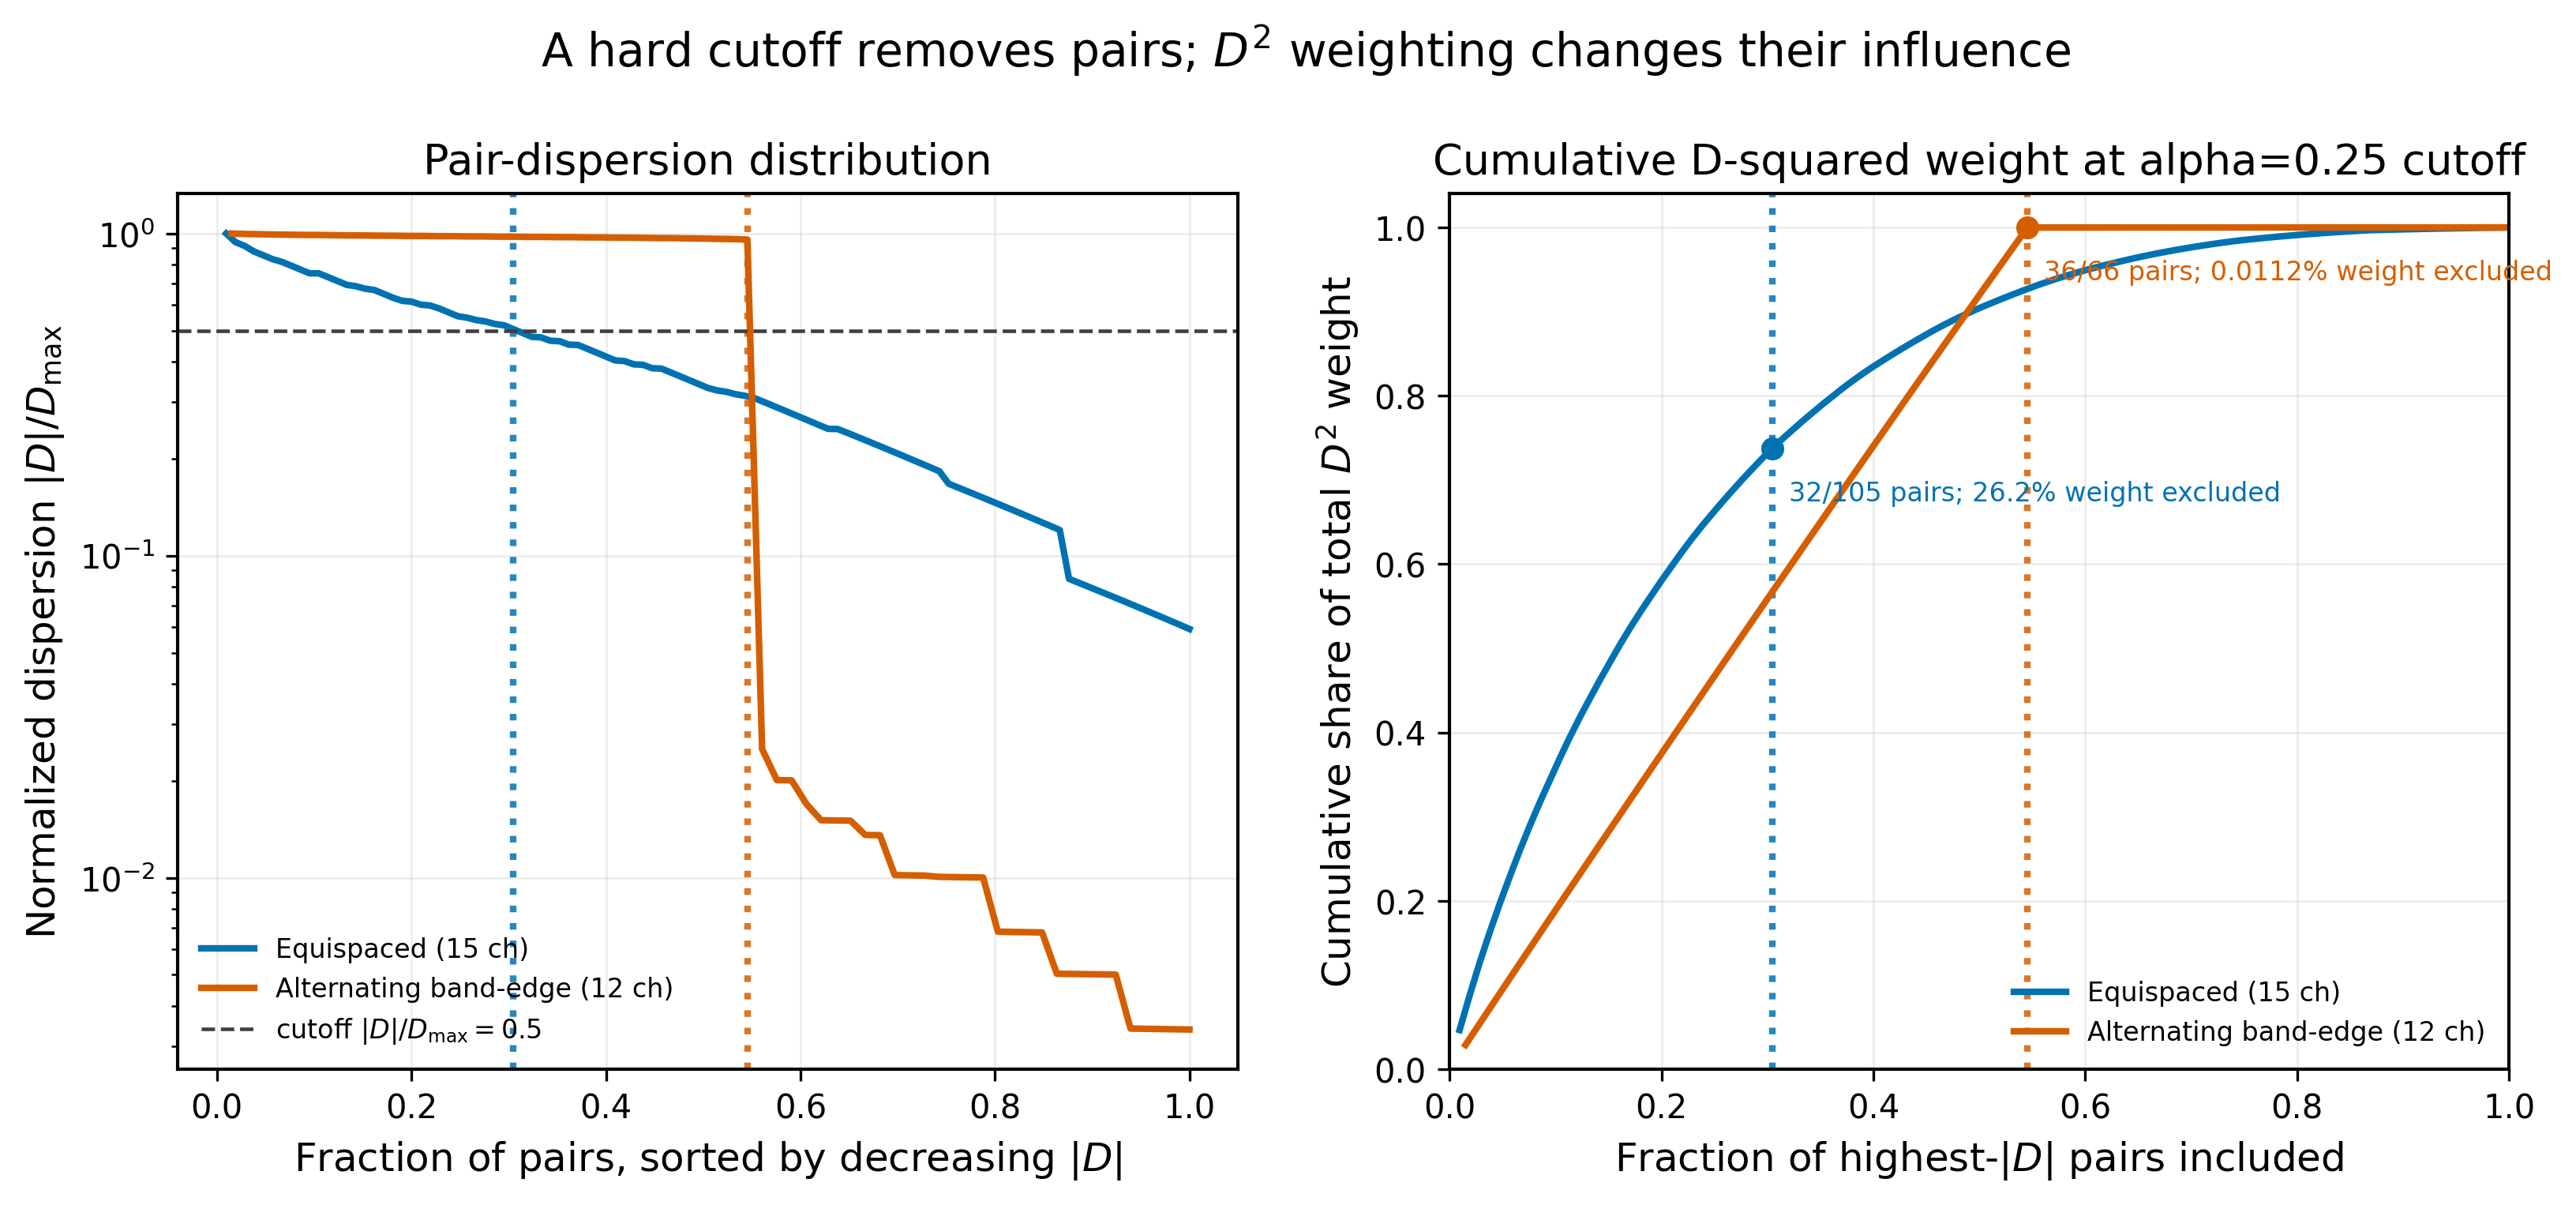
\includegraphics[width=0.90\linewidth]{F11_pair_weight_distribution.png}
\caption{Pair-dispersion distributions and cumulative $D^2$ weight. A graded equispaced grid retains appreciable weight below the hard cutoff; the band-edge layout nearly separates useful and weak pairs.}
\label{fig:weights}
\end{figure}

\section{Estimator choice, implications, and limits}
Fusion cannot repair every pair-delay estimator failure. Figure~\ref{fig:estimators} compares parabolic peak interpolation with generalized cross-correlation with phase transform (GCC-PHAT) \cite{knapp1976}, both under robust fusion. Their ranking changes with bandwidth and SNR. Near $22$\,kHz and 127.8\,dB, the 15-channel RMSE was 2.64\,km for parabolic and 0.71\,km for GCC-PHAT; near $1.3$\,kHz and 103.8\,dB, parabolic was better (25.8 versus 52.3\,km). Parabolic interpolation often has lower variance but can retain a bias floor; GCC-PHAT can reduce that bias but is not universally unbiased or robust to weak spectral bins. Accordingly, RMSE—not variance alone—is reported.

\begin{figure}[tb]
\centering
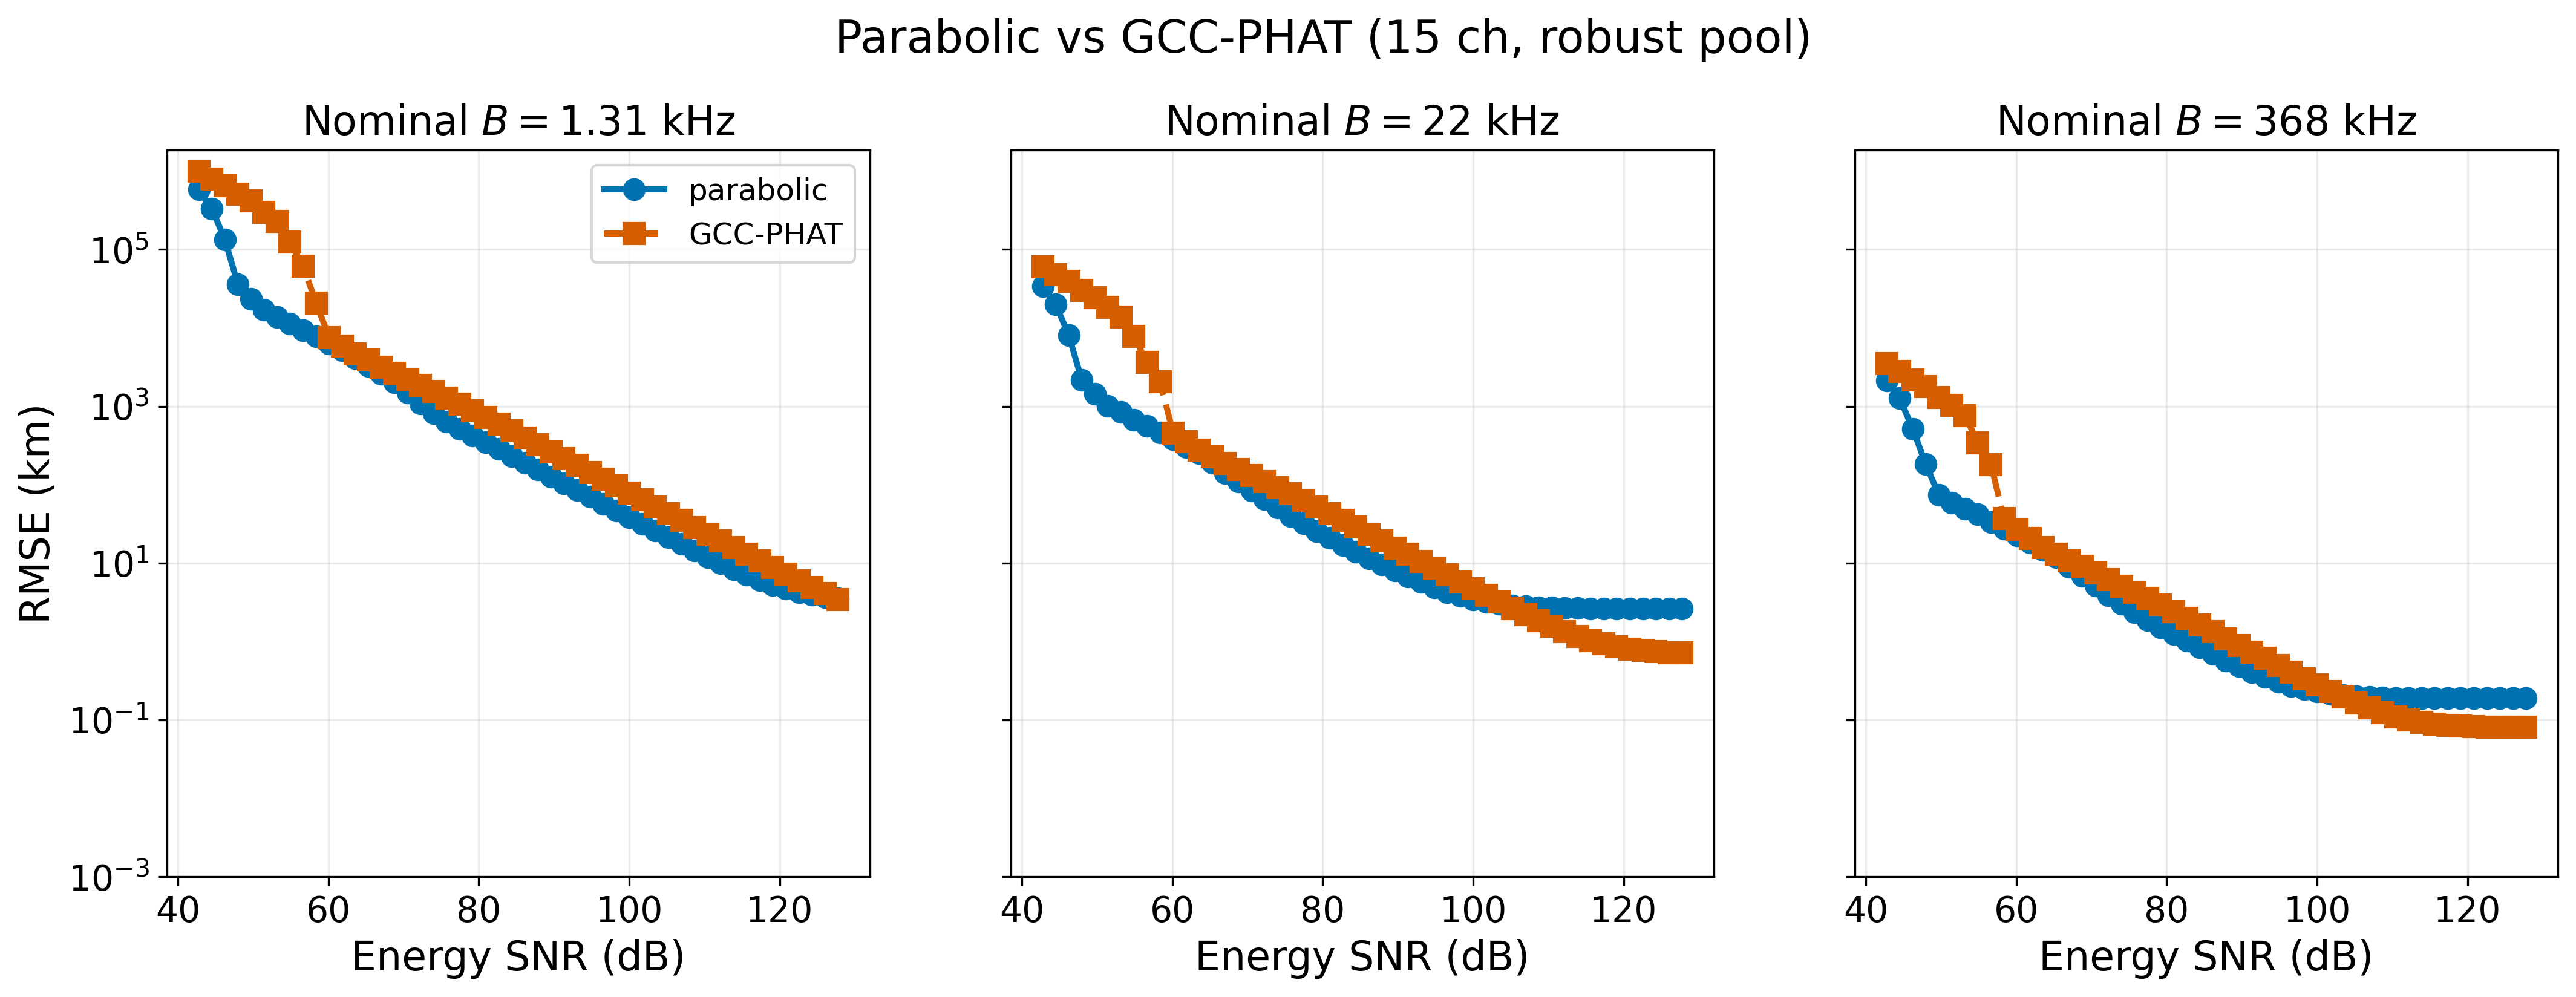
\includegraphics[width=0.90\linewidth]{F1_estimators_compare.png}
\caption{Parabolic and GCC-PHAT RMSE after the same robust fusion on an equispaced 15-channel grid. The crossover depends on bandwidth and SNR; neither estimator dominates throughout.}
\label{fig:estimators}
\end{figure}

The tested high-SNR spread approximately follows $\sigma_Z\propto(\sqrt{\SNR_E}B_{\rm nom})^{-1}$; more channels often reduce the SNR required for a target error, while averaging independent fibre realizations reduces spread approximately as $N_{\rm fib}^{-1/2}$. These are empirical scaling trends, not universal laws. The results support a practical sequence: confirm cross-channel observability, inspect the pair-dispersion distribution, compare equal, $D^2$, and robust fusion, and select the delay estimator using both bias and spread. Pair overlap precludes treating the $N(N-1)/2$ estimates as independent.

This is a simulation study of one localized SOP-perturbation model, with additive white independent noise and no experimental validation. Distributed PMD outside the local section, receiver imperfections, dispersion-calibration uncertainty, and paired confidence intervals remain future work. The main conclusion is conditional: WDM diversity can improve localization, but the gain depends on wavelength placement, estimator behavior, and fusion; no universal combined-CRB attainment is claimed.

\begin{thebibliography}{9}\footnotesize
\bibitem{he2021das} Z. He and Q. Liu, ``Optical fiber distributed acoustic sensors: A review,'' \emph{J. Lightwave Technol.} \textbf{39}(12), 3671--3686 (2021).
\bibitem{weiss1983} A. J. Weiss and E. Weinstein, ``Fundamental limitations in passive time-delay estimation---Part I: Narrowband systems,'' \emph{IEEE Trans. Acoust., Speech, Signal Process.} \textbf{31}(2), 472--485 (1983).
\bibitem{sadler2006survey} B. M. Sadler and R. J. Kozick, ``A survey of time delay estimation performance bounds,'' in \emph{Proc. Fourth IEEE Workshop on Sensor Array and Multichannel Processing}, 282--288 (2006).
\bibitem{gisin1992} N. Gisin and J. P. Pellaux, ``Polarization mode dispersion: time versus frequency domains,'' \emph{Opt. Commun.} \textbf{89}(2--4), 316--323 (1992).
\bibitem{knapp1976} C. Knapp and G. Carter, ``The generalized correlation method for estimation of time delay,'' \emph{IEEE Trans. Acoust., Speech, Signal Process.} \textbf{24}(4), 320--327 (1976).
\end{thebibliography}

\end{document}
